\documentclass{cumcmthesis1}
% \documentclass[withoutpreface,bwprint]{cumcmthesis} %去掉封面与编号页,电子版提交的时候使用。


\usepackage[framemethod=TikZ]{mdframed}
\usepackage{url}   % 网页链接
\usepackage{subcaption} % 子标题
\title{全国大学生数学建模竞赛编写的 \LaTeX{} 模板}
\tihao{A}
\baominghao{4321}
\schoolname{XX大学}
\membera{ }
\memberb{ }
\memberc{ }
\supervisor{ }
\yearinput{2024}
\monthinput{09}
\dayinput{22}

\begin{document}

 \maketitle
 \begin{abstract}
cumcmthesis 是为全国大学生数学建模竞赛编写的\LaTeX{}模板, 旨在让大家专注于 论文的内容写作, 而不用花费过多精力在格式的定制和调整上. 本手册是相应的参考, 其 中提供了一些环境和命令可以让模板的使用更为方便. 同时需要注意, 使用者需要有一 定的 \LaTeX{} 的使用经验, 至少要会使用常用宏包的一些功能, 比如参考文献,数学公式,图片使用,列表环境等等. 例子文件参看 \texttt{example.tex}.
2222222
\begin{mdframed} [%
	roundcorner=5pt,
	linecolor=gray!50,
	outerlinewidth=0.5pt,
	middlelinewidth=0.3pt, backgroundcolor=gray!2,
innertopmargin=\topskip, frametitle={2020 年建模比赛格式变化说明},
frametitlefont= \bfseries,frametitlerule=true,frametitlealignment =\raggedright\noindent,
frametitlerulewidth=.5pt, frametitlebackgroundcolor=gray!2,]
今年的格式变化主要就是三个地方,如下:


\end{mdframed}


\url{https://www.latexstudio.net} 陆续推出了更优质的资源,欢迎学习 。

欢迎大家到QQ群里沟通交流:91940767/478023327/640633524。我们也开通了问答区交流 \LaTeX{}技术:\url{https://ask.latexstudio.net},欢迎大家前来交流,有问题就来这里,与大神零距离。

\uwave{关注我们的微信公众号}:

\centerline{
\includegraphics[width=6cm]{gongzhonghao2}}

\keywords{\TeX{}\quad  图片\quad   表格\quad  公式}
\end{abstract}

%目录  2019 明确不要目录,我觉得这个规定太好了
%\tableofcontents

%\newpage

\section{模板的基本使用}

要使用 \LaTeX{} 来完成建模论文,首先要确保正确安装一个 \LaTeX{} 的发行版本。

\begin{itemize}
    \item Mac 下可以使用 Mac\TeX{}
    \item Linux 下可以使用 \TeX{}Live ;
    \item windows 下可以使用 \TeX{}Live 或者 Mik\TeX{} ;
\end{itemize}

具体安装可以参考 \href{https://github.com/OsbertWang/install-latex-guide-zh-cn/releases/}{Install-LaTeX-Guide-zh-cn} 或者其它靠谱的文章。另外可以安装一个易用的编辑器,例如 \href{https://mirrors.tuna.tsinghua.edu.cn/github-release/texstudio-org/texstudio/LatestRelease/}{\TeX{}studio} 。

使用该模板前,请阅读模板的使用说明文档。下面给出模板使用的大概样式。

\begin{tcode}
    \documentclass{cumcmthesis}
    \documentclass[withoutpreface,bwprint]{cumcmthesis} %去掉封面与编号页

    \title{论文题目}
    \tihao{A}            % 题号
    \baominghao{4321}    % 报名号
    \schoolname{你的大学}
    \membera{成员A}
    \memberb{成员B}
    \memberc{成员C}
    \supervisor{指导老师}
    \yearinput{2024}     % 年
    \monthinput{09}      % 月
    \dayinput{22}        % 日

    \begin{document}
        \maketitle
        \begin{abstract}
            摘要的具体内容。
            \keywords{关键词1\quad  关键词2\quad   关键词3}
        \end{abstract}
        \tableofcontents
        \section{问题重述}
        \subsection{问题的提出}
        \section{模型的假设}
        \section{符号说明}
        \begin{center}
            \begin{tabular}{cc}
                \hline
                \makebox[0.3\textwidth][c]{符号}	&  \makebox[0.4\textwidth][c]{意义} \\ \hline
                D	    & 木条宽度(cm) \\ \hline
            \end{tabular}
        \end{center}
        \section{问题分析}
        \section{总结}
        \begin{thebibliography}{9}%宽度9
            \bibitem{bib:one} ....
        \end{thebibliography}
        \begin{appendices}
            附录的内容。
        \end{appendices}
    \end{document}
\end{tcode}

根据要求,电子版论文提交时需去掉封面和编号页。可以加上 \verb|withoutpreface|  选项来实现,即:
\begin{tcode}
    \documentclass[withoutpreface]{cumcmthesis}
\end{tcode}
这样就能实现了。打印的时候有超链接的地方不需要彩色,可以加上 \verb|bwprint| 选项。

另外目录也是不需要的,将 \verb|\tableofcontents| 注释或删除,目录就不会出现了。

团队的信息填入指定的位置,并且确保信息的正确性,以免因此白忙一场。

编译记得使用 \verb|xelatex|,而不是用 \verb|pdflatex|。在命令行编译的可以按如下方式编译:
\begin{tcode}
	xelatex example
\end{tcode}
或者使用 \verb|latexmk| 来编译,更推荐这种方式。
\begin{tcode}
	latexmk -xelatex example
\end{tcode}

下面给出写作与排版上的一些建议。

\section{图片}

建模中不可避免要插入图片。图片可以分为矢量图与位图。位图推荐使用 \verb|jpg,png| 这两种格式,避免使用 \verb|bmp| 这类图片,容易出现图片插入失败这样情况的发生。矢量图一般有 \verb|pdf,eps| ,推荐使用 \verb|pdf|  格式的图片,尽量不要使用 \verb|eps| 图片,理由相同。

注意图片的命名,避免使用中文来命名图片,可以用英文与数字的组合来命名图片。避免使用\verb|1,2,3| 这样顺序的图片命名方式。图片多了,自己都不清楚那张图是什么了,命名尽量让它有意义。下面是一个插图的示例代码。
\begin{figure}[!h]
    \centering
    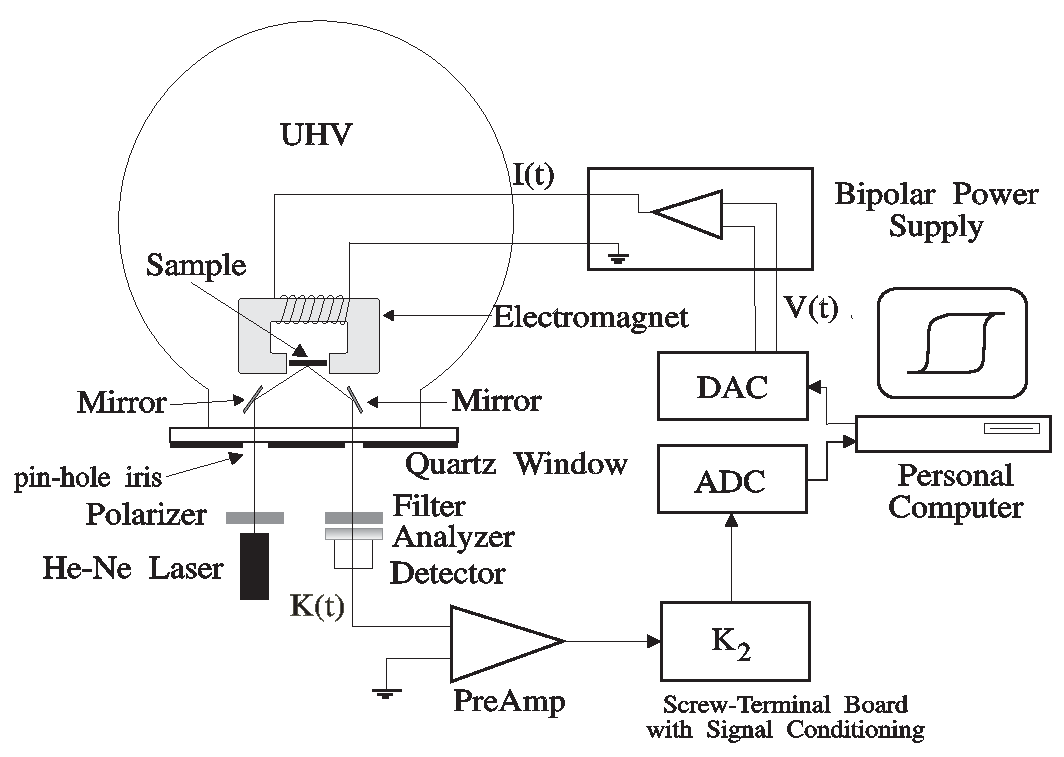
\includegraphics[width=.6\textwidth]{smokeblk}
    \caption{电路图}
    \label{fig:circuit-diagram}
\end{figure}

注意 \verb|figure| 环境是一个浮动体环境,图片的最终位置可能会跑动。\verb|[!h]| 中的 \verb|h| 是 here 的意思, \verb|!| 表示忽略一些浮动体的严格规则。另外里面还可以加上 \verb|btp| 选项,它们分别是 bottom, top, page 的意思。只要这几个参数在花括号里面,作用是不分先后顺序的。page 在这里表示浮动页。

\verb|\label{fig:circuit-diagram}| 是一个标签,供交叉引用使用的。例如引用图片 \verb|\cref{fig:circuit-diagram}| 的实际效果是\cref{fig:circuit-diagram}。图片是自动编号的,比起手动编号,它更加高效。\verb|\cref{label}| 由 \verb|cleveref| 宏包提供,比普通的 \verb|\ref{label}| 更加自动化。 \verb|label| 要确保唯一,命名方式推荐用图片的命名方式。

图片并排的需求解决方式多种多样,下面用 \verb|minipage| 环境来展示一个简单的例子。注意,以下例子用到了 \verb|subcaption| 命令,需要加载 subcaption 宏包。

\begin{figure}
    \centering
    \begin{minipage}[c]{0.3\textwidth}
        \centering
        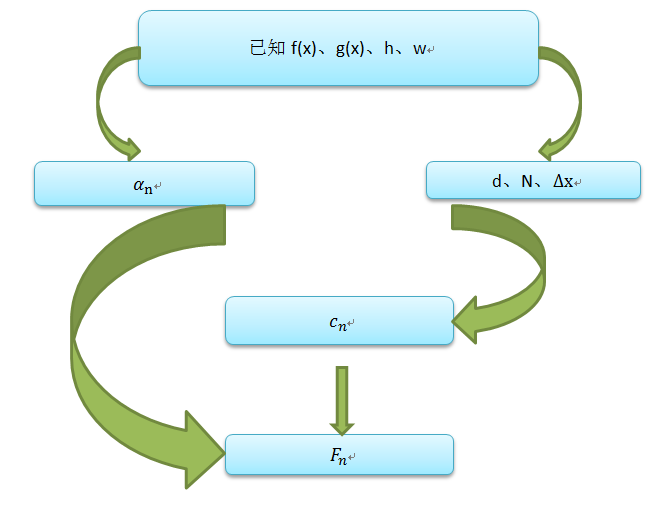
\includegraphics[width=0.95\textwidth]{f1}
        \subcaption{流程图}
        \label{fig:sample-figure-a}
    \end{minipage}
    \begin{minipage}[c]{0.3\textwidth}
        \centering
        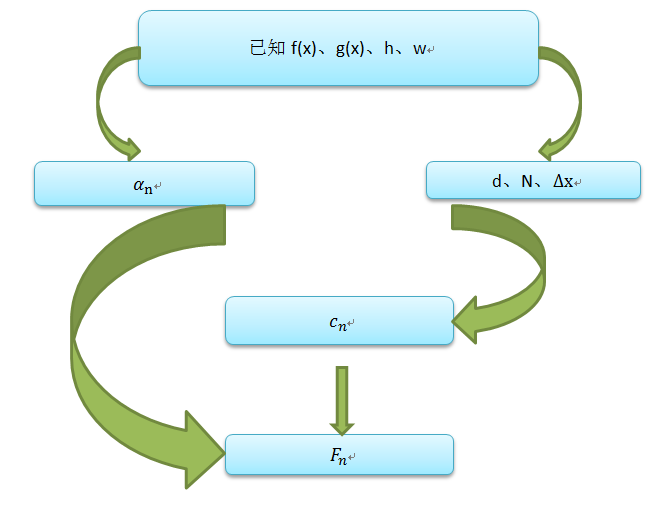
\includegraphics[width=0.95\textwidth]{f1}
        \subcaption{流程图}
        \label{fig:sample-figure-b}
    \end{minipage}
    \begin{minipage}[c]{0.3\textwidth}
        \centering
        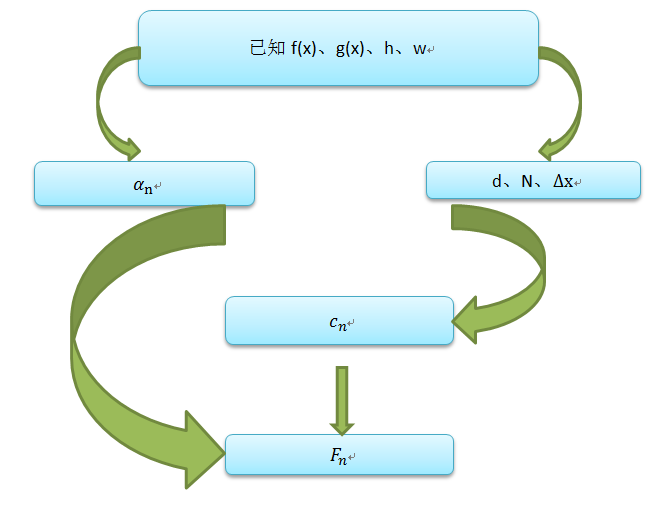
\includegraphics[width=0.95\textwidth]{f1}
        \subcaption{流程图}
        \label{fig:sample-figure-c}
    \end{minipage}
    \caption{多图并排示例}
    \label{fig:sample-figure}
\end{figure}
这相当于整体是一张大图片,大图片引用是\cref{fig:sample-figure},子图引用别分是\cref{fig:sample-figure-a}、\cref{fig:sample-figure-b}、\cref{fig:sample-figure-c}。

如果原本两张图片的高度不同,但是希望它们缩放后等高的排在同一行,参考这个例子:
\begin{figure}
    \centering
    \begin{minipage}[c]{0.48\textwidth}
        \centering
        
\includegraphics[height=0.2\textheight]{cat}
        \subcaption{一只猫}
    \end{minipage}
    \begin{minipage}[c]{0.48\textwidth}
        \centering
        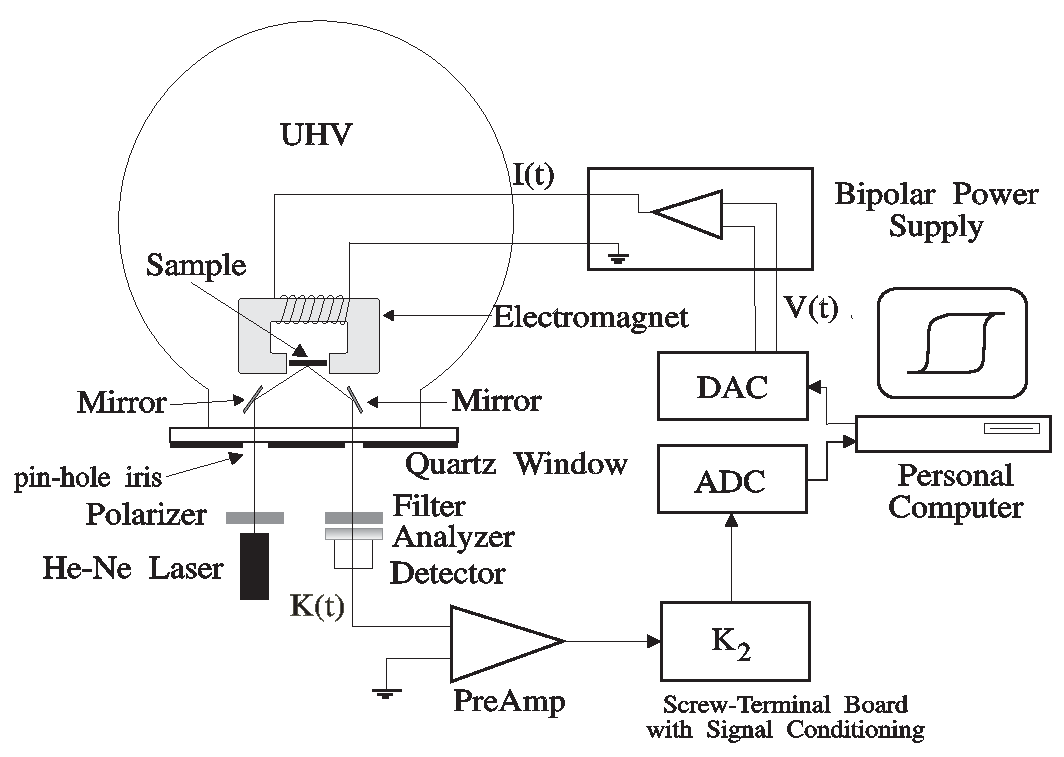
\includegraphics[height=0.2\textheight]{smokeblk}
        \subcaption{电路图}
    \end{minipage}
    \caption{多图并排示例}
\end{figure}

\section{绘制普通三线表格}
表格应具有三线表格式,因此常用 booktabs宏包,其标准格式如\cref{tab:001}~所示。
\begin{table}[!htbp]
    \caption{标准三线表格}\label{tab:001} \centering
    \begin{tabular}{ccccc}
        \toprule[1.5pt]
        $D$(in) & $P_u$(lbs) & $u_u$(in) & $\beta$ & $G_f$(psi.in)\\
        \midrule[1pt]
        5 & 269.8 & 0.000674 & 1.79 & 0.04089\\
        10 & 421.0 & 0.001035 & 3.59 & 0.04089\\
        20 & 640.2 & 0.001565 & 7.18 & 0.04089\\
        \bottomrule[1.5pt]
    \end{tabular}
\end{table}

其绘制表格的代码及其说明如下。
\begin{tcode}
    \begin{table}[!htbp]
        \caption[标签名]{中文标题}
        \begin{tabular}{cc...c}
            \toprule[1.5pt]
            表头第1个格   & 表头第2个格   & ... & 表头第n个格  \\
            \midrule[1pt]
            表中数据(1,1) & 表中数据(1,2) & ... & 表中数据(1,n)\\
            表中数据(2,1) & 表中数据(2,2) & ... & 表中数据(2,n)\\
            ...................................................\\
            表中数据(m,1) & 表中数据(m,2) & ... & 表中数据(m,n)\\
            \bottomrule[1.5pt]
        \end{tabular}
    \end{table}
\end{tcode}

\bigskip

table环境是一个将表格嵌入文本的浮动环境。tabular环境的必选参数由每列对应一个格式字符所组成:c表示居中,l表示左对齐,r表示右对齐,其总个数应与表的列数相同。此外,\verb|@{文本}|可以出现在任意两个上述的列格式之间,其中的文本将被插入每一行的同一位置。表格的各行以\verb|\\|分隔,同一行的各列则以\&分隔。 \verb|\toprule| 、\verb|\midrule| 和 \verb|\bottomrule| 三个命令是由booktabs宏包提供的,其中 \verb|\toprule| 和 \verb|\bottomrule| 分别用来绘制表格的第一条(表格最顶部)和第三条(表格最底部)水平线, \verb|\midrule| 用来绘制第二条(表头之下)水平线,且第一条和第三条水平线的线宽为 1.5pt ,第二条水平线的线宽为 1pt 。引用方法与图片的相同。

\section{公式}

数学建模必然涉及不少数学公式的使用。下面简单介绍一个可能用得上的数学环境。

首先是行内公式,例如 $ \theta $ 是角度。行内公式使用 \verb|$  $| 包裹。

行间公式不需要编号的可以使用 \verb|\[  \]| 包裹,例如
\[
E=mc^2
\]
其中 $ E $ 是能量,$ m $ 是质量,$ c $ 是光速。

如果希望某个公式带编号,并且在后文中引用可以参考下面的写法:
\begin{equation}
E=mc^2
\label{eq:energy}
\end{equation}
式\cref{eq:energy}是质能方程。

多行公式有时候希望能够在特定的位置对齐,以下是其中一种处理方法。
\begin{align}
P & = UI \\
& = I^2R
\end{align}
\verb|&| 是对齐的位置, \verb|&| 可以有多个,但是每行的个数要相同。

矩阵的输入也不难。
\[
\mathbf{X} = \left(
    \begin{array}{cccc}
    x_{11} & x_{12} & \ldots & x_{1n}\\
    x_{21} & x_{22} & \ldots & x_{2n}\\
    \vdots & \vdots & \ddots & \vdots\\
    x_{n1} & x_{n2} & \ldots & x_{nn}\\
    \end{array} \right)
\]

分段函数这些可以用 \verb|case| 环境,但是它要放在数学环境里面。
\[
f(x) =
    \begin{cases}
        0 &  x \text{为无理数} ,\\
        1 &  x \text{为有理数} .
    \end{cases}
\]
在数学环境里面,字体用的是数学字体,一般与正文字体不同。假如要公式里面有个别文字,则需要把这部分放在 \verb|text| 环境里面,即 \verb|\text{文本环境}| 。

公式中个别需要加粗的字母可以用 \verb|$\bm{math symbol}$| 。如 $ \alpha a\bm{\alpha a} $ 。

以上仅简单介绍了基础的使用,对于更复杂的需求,可以阅读相关的宏包手册,如 \href{http://texdoc.net/texmf-dist/doc/latex/amsmath/amsldoc.pdf}{amsmath}。

希腊字母这些如果不熟悉,可以去查找符号文件 \href{http://mirrors.ctan.org/info/symbols/comprehensive/symbols-a4.pdf}{symbols-a4.pdf} ,也可以去 \href{http://detexify.kirelabs.org/classify.html}{detexify} 网站手写识别。另外还有数学公式识别软件 \href{https://mathpix.com/}{mathpix} 。

下面简单介绍一下定理、证明等环境的使用。
\begin{definition}
    定义环境
    \label{def:nosense}
\end{definition}
\cref{def:nosense}除了告诉你怎么使用这个环境以外,没有什么其它的意义。

除了 definition 环境,还可以使用 theorem 、lemma、corollary、assumption、conjecture、axiom、principle、problem、example、proof、solution 这些环境,根据论文的实际需求合理使用。

\begin{theorem}
    这是一个定理。
    \label{thm:example}
\end{theorem}
由\cref{thm:example}我们知道了定理环境的使用。

\begin{lemma}
    这是一个引理。
    \label{lem:example}
\end{lemma}
由\cref{lem:example}我们知道了引理环境的使用。

\begin{corollary}
    这是一个推论。
    \label{cor:example}
\end{corollary}
由\cref{cor:example}我们知道了推论环境的使用。

\begin{assumption}
    这是一个假设。
    \label{asu:example}
\end{assumption}
由\cref{asu:example}我们知道了假设环境的使用。

\begin{conjecture}
    这是一个猜想。
    \label{con:example}
\end{conjecture}
由\cref{con:example}我们知道了猜想环境的使用。

\begin{axiom}
    这是一个公理。
    \label{axi:example}
\end{axiom}
由\cref{axi:example}我们知道了公理环境的使用。

\begin{principle}
    这是一个定律。
    \label{pri:example}
\end{principle}
由\cref{pri:example}我们知道了定律环境的使用。

\begin{problem}
    这是一个问题。
    \label{pro:example}
\end{problem}
由\cref{pro:example}我们知道了问题环境的使用。

\begin{example}
    这是一个例子。
    \label{exa:example}
\end{example}
由\cref{exa:example}我们知道了例子环境的使用。

\begin{proof}
    这是一个证明。
    \label{prf:example}
\end{proof}
由\cref{prf:example}我们知道了证明环境的使用。

\begin{solution}
    这是一个解。
    \label{sol:example}
\end{solution}
由\cref{sol:example}我们知道了解环境的使用。



\section{其它小功能}
\subsection{脚注}

利用 \verb|\footnote{具体内容}| 可以生成脚注\footnote{脚注可以补充说明一些东西}。

\subsection{无序列表与有序列表}

无序列表是这样的:
\begin{itemize}
    \item one
    \item two
    \item ...
\end{itemize}

有序列表是这样子的:
\begin{enumerate}
    \item one
    \item two
    \item ...
\end{enumerate}

\subsection{字体加粗与斜体}

如果想强调部分内容,可以使用加粗的手段来实现。加粗字体可以用 \verb|\textbf{加粗}| 来实现。例如: \textbf{这是加粗的字体。 This is bold fonts} 。

中文字体没有斜体设计,但是英文字体有。\textit{斜体 Italics}。

\section{参考文献与引用}

参考文献对于一篇正式的论文来说是必不可少的,在建模中重要的参考文献当然应该列出。\LaTeX{}在这方面的功能也是十分强大的,下面进介绍一个比较简单的参考文献制作方法。有兴趣的可以学习 \verb|bibtex| 或 \verb|biblatex| 的使用。

\LaTeX{}的入门书籍可以看《\LaTeX{}入门》\cite{liuhaiyang2013latex}。这是一个简单的引用,用 \verb|\cite{bibkey}| 来完成。要引用成功,当然要维护好 bibitem 了。下面是个简单的例子。



%参考文献
\begin{thebibliography}{9}%宽度9
    \bibitem[1]{liuhaiyang2013latex}
    刘海洋.
    \newblock \LaTeX {}入门\allowbreak[J].
    \newblock 电子工业出版社, 北京, 2013.
    \bibitem[2]{mathematical-modeling}
    全国大学生数学建模竞赛论文格式规范 (2020 年 8 月 25 日修改).
    \bibitem{3} \url{https://www.latexstudio.net}
\end{thebibliography}

\newpage
%附录
\begin{appendices}

\section{模板所用的宏包}
\begin{table}[htbp]
    \centering
    \caption{宏包罗列}
    \begin{tabular}{ccccc}
        \toprule
        \multicolumn{5}{c}{模板中已经加载的宏包} \\
        \midrule
        amsbsy & amsfonts & {amsgen} & {amsmath} & {amsopn} \\
        amssymb & amstext & {appendix} & {array} & {atbegshi} \\
        atveryend & auxhook & {bigdelim} & {bigintcalc} & {bigstrut} \\
        bitset & bm    & {booktabs} & {calc} & {caption} \\
        caption3 & CJKfntef & {cprotect} & {ctex} & {ctexhook} \\
        ctexpatch & enumitem & {etexcmds} & {etoolbox} & {everysel} \\
        expl3 & fix-cm & {fontenc} & {fontspec} & {fontspec-xetex} \\
        geometry & gettitlestring & {graphics} & {graphicx} & {hobsub} \\
        hobsub-generic & hobsub-hyperref & {hopatch} & {hxetex} & {hycolor} \\
        hyperref & ifluatex & {ifpdf} & {ifthen} & {ifvtex} \\
        ifxetex & indentfirst & {infwarerr} & {intcalc} & {keyval} \\
        kvdefinekeys & kvoptions & {kvsetkeys} & {l3keys2e} & {letltxmacro} \\
        listings & longtable & {lstmisc} & {ltcaption} & {ltxcmds} \\
        multirow & nameref & {pdfescape} & {pdftexcmds} & {refcount} \\
        rerunfilecheck & stringenc & {suffix} & {titletoc} & {tocloft} \\
        trig  & ulem  & {uniquecounter} & {url} & {xcolor} \\
        xcolor-patch & xeCJK & {xeCJKfntef} & {xeCJK-listings} & {xparse} \\
        xtemplate & zhnumber &       &       &  \\
        \bottomrule
    \end{tabular}%
    \label{tab:addlabel}%
\end{table}%

以上宏包都已经加载过了,不要重复加载它们。

\section{排队算法--matlab 源程序}

\begin{lstlisting}[language=matlab]
kk=2;[mdd,ndd]=size(dd);
while ~isempty(V)
[tmpd,j]=min(W(i,V));tmpj=V(j);
for k=2:ndd
[tmp1,jj]=min(dd(1,k)+W(dd(2,k),V));
tmp2=V(jj);tt(k-1,:)=[tmp1,tmp2,jj];
end
tmp=[tmpd,tmpj,j;tt];[tmp3,tmp4]=min(tmp(:,1));
if tmp3==tmpd, ss(1:2,kk)=[i;tmp(tmp4,2)];
else,tmp5=find(ss(:,tmp4)~=0);tmp6=length(tmp5);
if dd(2,tmp4)==ss(tmp6,tmp4)
ss(1:tmp6+1,kk)=[ss(tmp5,tmp4);tmp(tmp4,2)];
else, ss(1:3,kk)=[i;dd(2,tmp4);tmp(tmp4,2)];
end;end
dd=[dd,[tmp3;tmp(tmp4,2)]];V(tmp(tmp4,3))=[];
[mdd,ndd]=size(dd);kk=kk+1;
end; S=ss; D=dd(1,:);
 \end{lstlisting}

 \section{规划解决程序--lingo源代码}

\begin{lstlisting}[language=c]
kk=2;
[mdd,ndd]=size(dd);
while ~isempty(V)
    [tmpd,j]=min(W(i,V));tmpj=V(j);
for k=2:ndd
    [tmp1,jj]=min(dd(1,k)+W(dd(2,k),V));
    tmp2=V(jj);tt(k-1,:)=[tmp1,tmp2,jj];
end
    tmp=[tmpd,tmpj,j;tt];[tmp3,tmp4]=min(tmp(:,1));
if tmp3==tmpd, ss(1:2,kk)=[i;tmp(tmp4,2)];
else,tmp5=find(ss(:,tmp4)~=0);tmp6=length(tmp5);
if dd(2,tmp4)==ss(tmp6,tmp4)
    ss(1:tmp6+1,kk)=[ss(tmp5,tmp4);tmp(tmp4,2)];
else, ss(1:3,kk)=[i;dd(2,tmp4);tmp(tmp4,2)];
end;
end
    dd=[dd,[tmp3;tmp(tmp4,2)]];V(tmp(tmp4,3))=[];
    [mdd,ndd]=size(dd);
    kk=kk+1;
end;
S=ss;
D=dd(1,:);
 \end{lstlisting}
\end{appendices}

\end{document} 